\documentclass{standalone}
\usepackage{tikz}
\usetikzlibrary{patterns, positioning}

\begin{document}
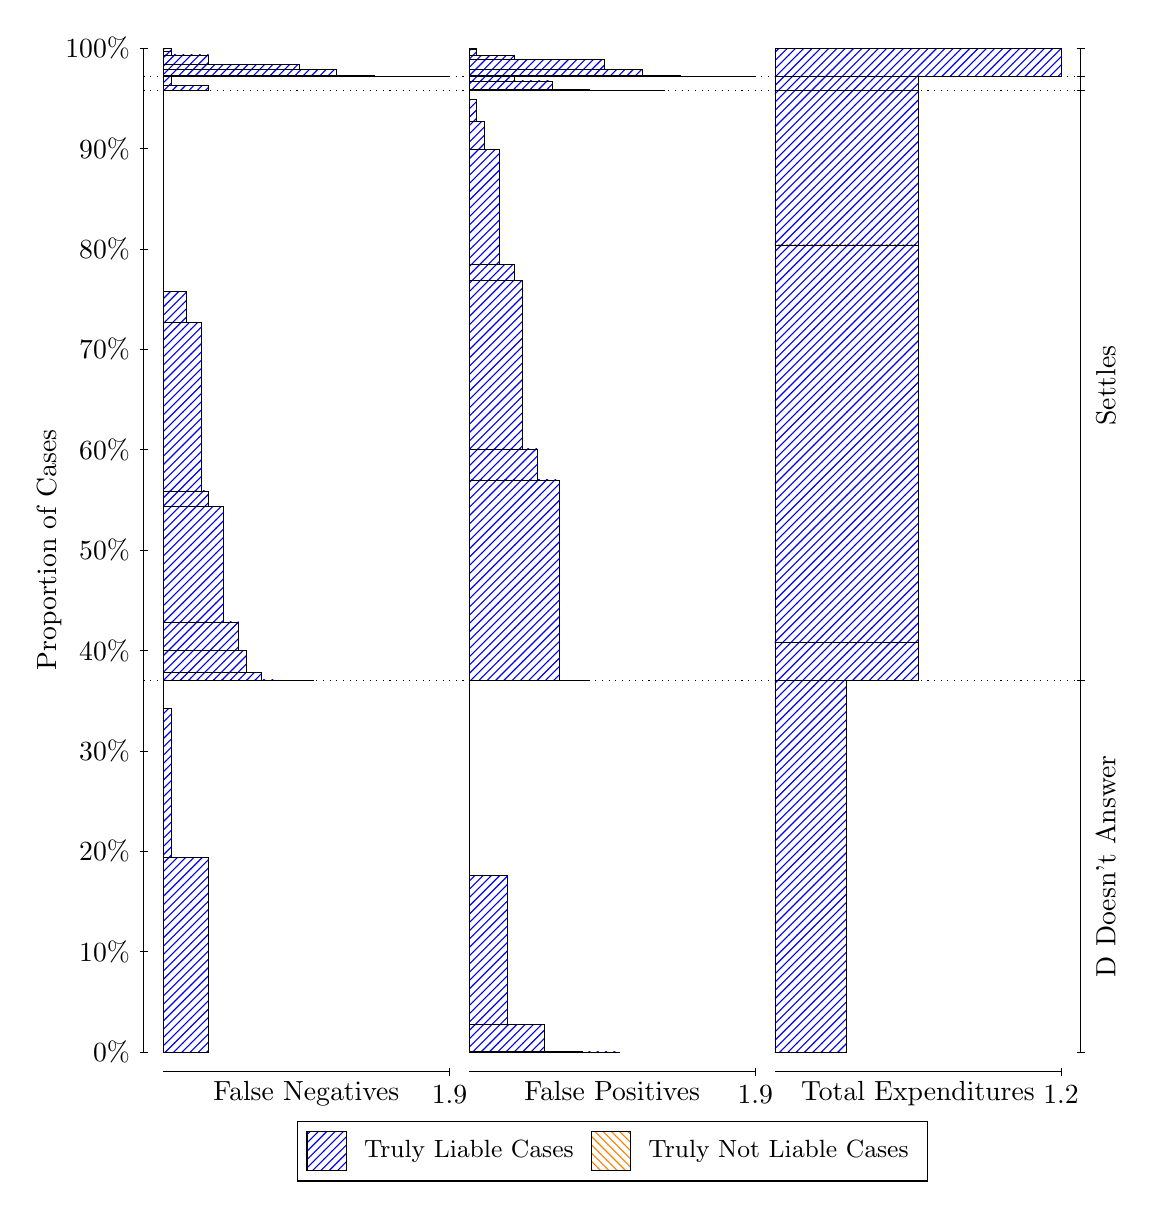
\begin{tikzpicture}
\draw[black, very thin] (1.5,1.75) -- (1.5,14.5);
\node[rotate=90, anchor=center] at (0.3, 8.125) {Proportion of Cases};
\draw[black, very thin] (1.45,1.75) -- (1.55,1.75);
\node[anchor=east] at (1.45, 1.75) {0\%};
\draw[black, very thin] (1.45,3.025) -- (1.55,3.025);
\node[anchor=east] at (1.45, 3.025) {10\%};
\draw[black, very thin] (1.45,4.3) -- (1.55,4.3);
\node[anchor=east] at (1.45, 4.3) {20\%};
\draw[black, very thin] (1.45,5.575) -- (1.55,5.575);
\node[anchor=east] at (1.45, 5.575) {30\%};
\draw[black, very thin] (1.45,6.85) -- (1.55,6.85);
\node[anchor=east] at (1.45, 6.85) {40\%};
\draw[black, very thin] (1.45,8.125) -- (1.55,8.125);
\node[anchor=east] at (1.45, 8.125) {50\%};
\draw[black, very thin] (1.45,9.4) -- (1.55,9.4);
\node[anchor=east] at (1.45, 9.4) {60\%};
\draw[black, very thin] (1.45,10.675) -- (1.55,10.675);
\node[anchor=east] at (1.45, 10.675) {70\%};
\draw[black, very thin] (1.45,11.95) -- (1.55,11.95);
\node[anchor=east] at (1.45, 11.95) {80\%};
\draw[black, very thin] (1.45,13.225) -- (1.55,13.225);
\node[anchor=east] at (1.45, 13.225) {90\%};
\draw[black, very thin] (1.45,14.5) -- (1.55,14.5);
\node[anchor=east] at (1.45, 14.5) {100\%};

\draw[black, very thin] (13.4,1.75) -- (13.4,14.5);
\draw[black, very thin] (13.35,1.75) -- (13.45,1.75);
\node[anchor=west] at (13.35, 1.75) {};
\draw[black, very thin] (13.35,6.4642) -- (13.45,6.4642);
\node[anchor=west] at (13.35, 6.4642) {};
\draw[black, very thin] (13.35,13.961) -- (13.45,13.961);
\node[anchor=west] at (13.35, 13.961) {};
\draw[black, very thin] (13.35,14.143) -- (13.45,14.143);
\node[anchor=west] at (13.35, 14.143) {};
\draw[black, very thin] (13.35,14.5) -- (13.45,14.5);
\node[anchor=west] at (13.35, 14.5) {};

\draw[black, very thin, pattern color=blue, pattern=north east lines] (1.75,1.75) rectangle (2.3237,4.226);
\draw[black, very thin, pattern color=blue, pattern=north east lines] (1.75,4.226) rectangle (1.8456,6.1154);
\draw[black, very thin, pattern color=orange, pattern=north west lines] (1.75,6.1154) rectangle (1.75,6.1154);
\draw[black, very thin, pattern color=blue, pattern=north east lines] (1.75,6.1154) rectangle (1.75,6.4642);
\draw[black, very thin, pattern color=blue, pattern=north east lines] (1.75,6.4642) rectangle (3.6623,6.4642);
\draw[black, very thin, pattern color=blue, pattern=north east lines] (1.75,6.4642) rectangle (3.4711,6.4643);
\draw[black, very thin, pattern color=blue, pattern=north east lines] (1.75,6.4643) rectangle (3.2798,6.4729);
\draw[black, very thin, pattern color=blue, pattern=north east lines] (1.75,6.4729) rectangle (3.1842,6.4744);
\draw[black, very thin, pattern color=blue, pattern=north east lines] (1.75,6.4744) rectangle (2.993,6.5755);
\draw[black, very thin, pattern color=blue, pattern=north east lines] (1.75,6.5755) rectangle (2.8018,6.854);
\draw[black, very thin, pattern color=blue, pattern=north east lines] (1.75,6.854) rectangle (2.7061,7.2122);
\draw[black, very thin, pattern color=blue, pattern=north east lines] (1.75,7.2122) rectangle (2.5149,8.6743);
\draw[black, very thin, pattern color=blue, pattern=north east lines] (1.75,8.6743) rectangle (2.3237,8.8748);
\draw[black, very thin, pattern color=blue, pattern=north east lines] (1.75,8.8748) rectangle (2.2281,11.016);
\draw[black, very thin, pattern color=blue, pattern=north east lines] (1.75,11.016) rectangle (2.0368,11.409);
\draw[black, very thin, pattern color=blue, pattern=north east lines] (1.75,11.409) rectangle (1.8456,11.411);
\draw[black, very thin, pattern color=orange, pattern=north west lines] (1.75,11.411) rectangle (1.75,11.411);
\draw[black, very thin, pattern color=blue, pattern=north east lines] (1.75,11.411) rectangle (1.75,13.961);
\draw[black, very thin, pattern color=blue, pattern=north east lines] (1.75,13.961) rectangle (2.3237,14.023);
\draw[black, very thin, pattern color=blue, pattern=north east lines] (1.75,14.023) rectangle (1.8456,14.135);
\draw[black, very thin, pattern color=orange, pattern=north west lines] (1.75,14.135) rectangle (1.75,14.135);
\draw[black, very thin, pattern color=blue, pattern=north east lines] (1.75,14.135) rectangle (1.75,14.143);
\draw[black, very thin, pattern color=blue, pattern=north east lines] (1.75,14.143) rectangle (5.3833,14.143);
\draw[black, very thin, pattern color=blue, pattern=north east lines] (1.75,14.143) rectangle (4.9053,14.144);
\draw[black, very thin, pattern color=blue, pattern=north east lines] (1.75,14.144) rectangle (4.4272,14.151);
\draw[black, very thin, pattern color=blue, pattern=north east lines] (1.75,14.151) rectangle (3.9491,14.233);
\draw[black, very thin, pattern color=blue, pattern=north east lines] (1.75,14.233) rectangle (3.4711,14.29);
\draw[black, very thin, pattern color=blue, pattern=north east lines] (1.75,14.29) rectangle (3.2798,14.29);
\draw[black, very thin, pattern color=blue, pattern=north east lines] (1.75,14.29) rectangle (2.993,14.29);
\draw[black, very thin, pattern color=blue, pattern=north east lines] (1.75,14.29) rectangle (2.8018,14.292);
\draw[black, very thin, pattern color=blue, pattern=north east lines] (1.75,14.292) rectangle (2.5149,14.292);
\draw[black, very thin, pattern color=blue, pattern=north east lines] (1.75,14.292) rectangle (2.3237,14.294);
\draw[black, very thin, pattern color=blue, pattern=north east lines] (1.75,14.294) rectangle (2.3237,14.414);
\draw[black, very thin, pattern color=blue, pattern=north east lines] (1.75,14.414) rectangle (1.8456,14.453);
\draw[black, very thin, pattern color=blue, pattern=north east lines] (1.75,14.453) rectangle (1.8456,14.496);
\draw[black, very thin, pattern color=orange, pattern=north west lines] (1.75,14.496) rectangle (1.75,14.496);
\draw[black, very thin, pattern color=blue, pattern=north east lines] (1.75,14.496) rectangle (1.75,14.5);
\draw[black, very thin, pattern color=orange, pattern=north west lines] (5.6333,1.75) rectangle (7.5456,1.75);
\draw[black, very thin, pattern color=blue, pattern=north east lines] (5.6333,1.75) rectangle (7.5456,1.75);
\draw[black, very thin, pattern color=blue, pattern=north east lines] (5.6333,1.75) rectangle (7.0675,1.7529);
\draw[black, very thin, pattern color=blue, pattern=north east lines] (5.6333,1.7529) rectangle (6.5895,2.0988);
\draw[black, very thin, pattern color=blue, pattern=north east lines] (5.6333,2.0988) rectangle (6.1114,3.9882);
\draw[black, very thin, pattern color=blue, pattern=north east lines] (5.6333,3.9882) rectangle (5.6333,6.4642);
\draw[black, very thin, pattern color=orange, pattern=north west lines] (5.6333,6.4642) rectangle (7.1632,6.4642);
\draw[black, very thin, pattern color=blue, pattern=north east lines] (5.6333,6.4642) rectangle (7.1632,6.4642);
\draw[black, very thin, pattern color=orange, pattern=north west lines] (5.6333,6.4642) rectangle (6.9719,6.4642);
\draw[black, very thin, pattern color=blue, pattern=north east lines] (5.6333,6.4642) rectangle (6.9719,6.4682);
\draw[black, very thin, pattern color=orange, pattern=north west lines] (5.6333,6.4682) rectangle (6.7807,6.4682);
\draw[black, very thin, pattern color=blue, pattern=north east lines] (5.6333,6.4682) rectangle (6.7807,9.0141);
\draw[black, very thin, pattern color=blue, pattern=north east lines] (5.6333,9.0141) rectangle (6.6851,9.0158);
\draw[black, very thin, pattern color=blue, pattern=north east lines] (5.6333,9.0158) rectangle (6.4939,9.4093);
\draw[black, very thin, pattern color=blue, pattern=north east lines] (5.6333,9.4093) rectangle (6.3026,11.55);
\draw[black, very thin, pattern color=blue, pattern=north east lines] (5.6333,11.55) rectangle (6.207,11.751);
\draw[black, very thin, pattern color=blue, pattern=north east lines] (5.6333,11.751) rectangle (6.0158,13.213);
\draw[black, very thin, pattern color=blue, pattern=north east lines] (5.6333,13.213) rectangle (5.8246,13.571);
\draw[black, very thin, pattern color=blue, pattern=north east lines] (5.6333,13.571) rectangle (5.7289,13.85);
\draw[black, very thin, pattern color=blue, pattern=north east lines] (5.6333,13.85) rectangle (5.6333,13.961);
\draw[black, very thin, pattern color=orange, pattern=north west lines] (5.6333,13.961) rectangle (8.1193,13.961);
\draw[black, very thin, pattern color=blue, pattern=north east lines] (5.6333,13.961) rectangle (8.1193,13.961);
\draw[black, very thin, pattern color=blue, pattern=north east lines] (5.6333,13.961) rectangle (7.6412,13.961);
\draw[black, very thin, pattern color=blue, pattern=north east lines] (5.6333,13.961) rectangle (7.1632,13.97);
\draw[black, very thin, pattern color=blue, pattern=north east lines] (5.6333,13.97) rectangle (6.6851,14.082);
\draw[black, very thin, pattern color=blue, pattern=north east lines] (5.6333,14.082) rectangle (6.207,14.143);
\draw[black, very thin, pattern color=orange, pattern=north west lines] (5.6333,14.143) rectangle (9.2667,14.143);
\draw[black, very thin, pattern color=blue, pattern=north east lines] (5.6333,14.143) rectangle (9.2667,14.143);
\draw[black, very thin, pattern color=orange, pattern=north west lines] (5.6333,14.143) rectangle (8.7886,14.143);
\draw[black, very thin, pattern color=blue, pattern=north east lines] (5.6333,14.143) rectangle (8.7886,14.143);
\draw[black, very thin, pattern color=orange, pattern=north west lines] (5.6333,14.143) rectangle (8.3105,14.143);
\draw[black, very thin, pattern color=blue, pattern=north east lines] (5.6333,14.143) rectangle (8.3105,14.148);
\draw[black, very thin, pattern color=blue, pattern=north east lines] (5.6333,14.148) rectangle (7.8325,14.23);
\draw[black, very thin, pattern color=blue, pattern=north east lines] (5.6333,14.23) rectangle (7.3544,14.352);
\draw[black, very thin, pattern color=orange, pattern=north west lines] (5.6333,14.352) rectangle (7.1632,14.352);
\draw[black, very thin, pattern color=blue, pattern=north east lines] (5.6333,14.352) rectangle (7.1632,14.352);
\draw[black, very thin, pattern color=blue, pattern=north east lines] (5.6333,14.352) rectangle (6.8763,14.353);
\draw[black, very thin, pattern color=orange, pattern=north west lines] (5.6333,14.353) rectangle (6.6851,14.353);
\draw[black, very thin, pattern color=blue, pattern=north east lines] (5.6333,14.353) rectangle (6.6851,14.354);
\draw[black, very thin, pattern color=blue, pattern=north east lines] (5.6333,14.354) rectangle (6.3982,14.354);
\draw[black, very thin, pattern color=blue, pattern=north east lines] (5.6333,14.354) rectangle (6.207,14.411);
\draw[black, very thin, pattern color=orange, pattern=north west lines] (5.6333,14.411) rectangle (6.207,14.411);
\draw[black, very thin, pattern color=blue, pattern=north east lines] (5.6333,14.411) rectangle (6.207,14.411);
\draw[black, very thin, pattern color=blue, pattern=north east lines] (5.6333,14.411) rectangle (5.7289,14.49);
\draw[black, very thin, pattern color=blue, pattern=north east lines] (5.6333,14.49) rectangle (5.7289,14.492);
\draw[black, very thin, pattern color=blue, pattern=north east lines] (5.6333,14.492) rectangle (5.6333,14.5);
\draw[black, very thin, pattern color=orange, pattern=north west lines] (9.5167,1.75) rectangle (10.425,1.75);
\draw[black, very thin, pattern color=blue, pattern=north east lines] (9.5167,1.75) rectangle (10.425,6.4642);
\draw[black, very thin, pattern color=orange, pattern=north west lines] (9.5167,6.4642) rectangle (11.333,6.4642);
\draw[black, very thin, pattern color=blue, pattern=north east lines] (9.5167,6.4642) rectangle (11.333,6.9535);
\draw[black, very thin, pattern color=orange, pattern=north west lines] (9.5167,6.9535) rectangle (11.333,6.9535);
\draw[black, very thin, pattern color=blue, pattern=north east lines] (9.5167,6.9535) rectangle (11.333,12);
\draw[black, very thin, pattern color=orange, pattern=north west lines] (9.5167,12) rectangle (11.333,12);
\draw[black, very thin, pattern color=blue, pattern=north east lines] (9.5167,12) rectangle (11.333,13.961);
\draw[black, very thin, pattern color=orange, pattern=north west lines] (9.5167,13.961) rectangle (11.333,13.961);
\draw[black, very thin, pattern color=blue, pattern=north east lines] (9.5167,13.961) rectangle (11.333,14.143);
\draw[black, very thin, pattern color=orange, pattern=north west lines] (9.5167,14.143) rectangle (13.15,14.143);
\draw[black, very thin, pattern color=blue, pattern=north east lines] (9.5167,14.143) rectangle (13.15,14.5);
\draw[black, dotted] (1.5,6.4642) -- (13.4,6.4642);
\draw[black, dotted] (1.5,13.961) -- (13.4,13.961);
\draw[black, dotted] (1.5,14.143) -- (13.4,14.143);
\draw[black, very thin] (1.75,1.5) -- (5.3833,1.5);
\node[anchor=north] at (3.5667, 1.5) {False Negatives};
\draw[black, very thin] (5.3833,1.45) -- (5.3833,1.55);
\node[anchor=north] at (5.3833, 1.45) {1.9};

\draw[black, very thin] (5.6333,1.5) -- (9.2667,1.5);
\node[anchor=north] at (7.45, 1.5) {False Positives};
\draw[black, very thin] (9.2667,1.45) -- (9.2667,1.55);
\node[anchor=north] at (9.2667, 1.45) {1.9};

\draw[black, very thin] (9.5167,1.5) -- (13.15,1.5);
\node[anchor=north] at (11.333, 1.5) {Total Expenditures};
\draw[black, very thin] (13.15,1.45) -- (13.15,1.55);
\node[anchor=north] at (13.15, 1.45) {1.2};

\node[black, centered, rotate=90] at (13.72, 4.1071) {D Doesn't Answer};
\node[black, centered, rotate=90] at (13.72, 10.213) {Settles};



\draw (7.449999999999999,1.5) node[draw=none] (baseCoordinate) {};
\begin{scope}[align=center]
        \matrix[scale=0.5, draw=black, below=0.5cm of baseCoordinate, nodes={draw}, column sep=0.1cm]{
            \node[rectangle, draw, minimum width=0.5cm, minimum height=0.5cm, pattern=north east lines, pattern color=blue] {}; &
            \node[draw=none, font=\small] (B) {Truly Liable Cases}; &
            \node[rectangle, draw, minimum width=0.5cm, minimum height=0.5cm, pattern=north west lines, pattern color=orange] {}; &
            \node[draw=none, font=\small] (B) {Truly Not Liable Cases}; \\
            };
\end{scope}

\end{tikzpicture}
\end{document}